\section{Literaturverwaltung}
\label{sec:literatur}

Um die ersten Studien- oder Abschlussarbeiten in \LaTeX\ zu setzen, fehlt uns jetzt nur noch eine Möglichkeit, Literatur zu referenzieren.
Unsere Literatursammlung liegt in der sogenannten .bib-Datei.
Wenn wir aus unserem \LaTeX-Dokument darauf verweisen, kann uns das Programm BibTeX (ähnlich zum Compiler PDFLaTeX) an der richtigen Stelle die richtigen Zitationen im vorher festgelegten Bibliografiestil einfügen.

\subsection{Die Bibliografie-Datei}
In der .bib-Datei sammeln wir unsere Literatureinträge in einem Format, das durch BibTeX verarbeitbar ist.
Einen beispielhaften Eintrag aus einer .bib-Datei zeigt \cref{lst:bibfile-sample-entry}.

\begin{figure}[H]
  \begin{minted}{latex}
  @article{turing1990, % Dokumentenart und Bezeichner für den \cite-Befehl
    title={The chemical basis of morphogenesis}, % Titel
    author={Turing, Alan Mathison}, % Autor
    journal={Bulletin of mathematical biology}, % Titel des Journals
    volume={52}, % Band des Journals
    pages={153--197}, % Seitenzahl im Journal
    year={1990}, % Erscheinungsjahr
    publisher={Springer} % Verleger des Journals
  }
  \end{minted}
  \caption{Beispielhafter Eintrag einer .bib-Datei}
  \label{lst:bibfile-sample-entry}
\end{figure}

Nach einem @-Zeichen wird die Art des Literaturverzeichniseintrags angegeben (z.\,B. article, book, proceedings).
Es folgt eine Auflistung wichtiger Attribute wie Titel, Autor:in und – abhängig vom Eintragstyp – weiterer Felder.
Der erste Eintrag nach der öffnenden geschwungenen Klammer ist der wichtigste: 
Unter diesem Kürzel wird der Eintrag später in LaTeX angesprochen.
Diese sogenannten BibTeX-Keys müssen eindeutig sein und können frei vergeben werden.
Üblich sind Kombinationen aus Autor:innen, Publikationsjahren und Themen.


Die .bib-Datei kann manuell zusammengetragen werden.
Viel häufiger allerdings werden dafür Programme wie JabRef\footnote{Vgl. \url{https://www.jabref.org/}}, Zotero\footnote{Vgl. \url{https://www.zotero.org/}} oder das weit verbreitete Citavi\footnote{Vgl. \url{https://www.citavi.com/de}} verwendet.
Während JabRef direkt eine .bib-Datei als Datenbank verwendet, lassen sich Zotero- und Citavi-Projekte\footnote{Vgl. \url{https://www1.citavi.com/sub/manual5/de/exporting_to_bibtex.html}} in .bib-Dateien exportieren.

.bib-Datei-Einträge werden unter anderem auch von Google Scholar zur Verfügung gestellt (vgl. \cref{fig:google-scholar-bibtex}).
Hierbei ist es wichtig, darauf zu achten, dass die Einträge einheitlich und möglichst vollständig sind.
Als hochwertige (wenn auch leider nicht vollständige) Quelle für BibTeX-Einträge kann die dblp Computer Science Library\footnote{Verfügbar unter \url{https://dblp.org/search}.} dienen.

\begin{figure}[H]
  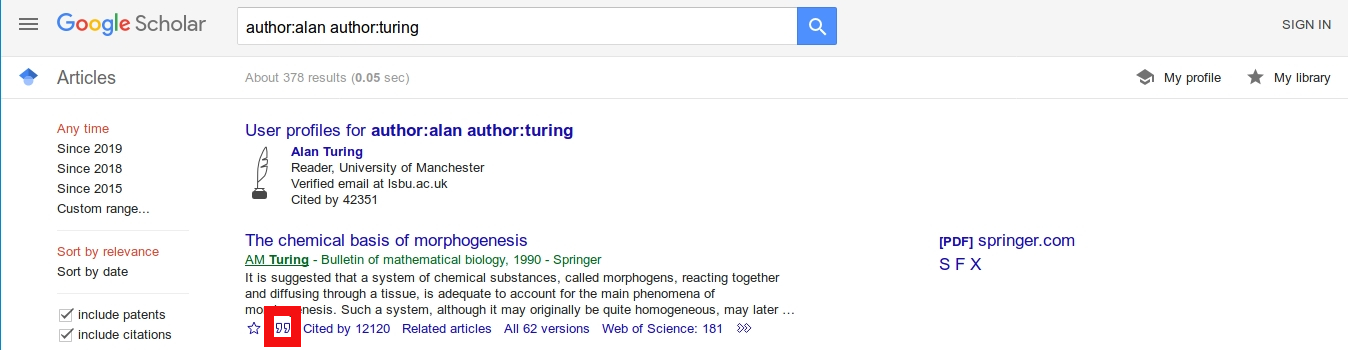
\includegraphics[width=\textwidth]{graphics/google_bibtex1.jpg}  
  
\includegraphics[width=\textwidth]{graphics/google_bibtex2.jpg}  
  \caption{BibTeX-Einträge in Google Scholar abrufen}
  \label{fig:google-scholar-bibtex}
\end{figure}

\subsection{Zitieren}
Durch BibTeX wird LaTeX um einige Befehle (vgl. \cref{tab:bibtex-commands}) zum Zitieren erweitert. 
Zusätzlich benötigt wird das Paket \mintinline{latex}{natbib}.

\begin{table}[H]
  \centering
  \begin{tabular}{ll}
  \toprule
  Funktion                 & Befehl \\ \midrule
  Quelle zitieren          & \mintinline{latex}{\cite{<quelle>}} \\
  Seite zitieren           & \mintinline{latex}{\cite[S. 15]{<quelle>}} \\
  Weitere Zusätze zitieren & \mintinline{latex}{\cite[<präfix>][<suffix>]{<quelle>}} \\
  .bib-Datei einbinden     & \mintinline{latex}{\bibliography{<.bib-datei>}} \\
  Zitierstil ändern        & \mintinline{latex}{\bibliographystyle{<zitierstil>}} \\ \bottomrule
  \end{tabular}
  \caption{Befehle zum Zitieren von Literatur}
  \label{tab:bibtex-commands}
\end{table}

Als \mintinline{latex}{<quelle>} wird immer der BibTeX-Key angegeben.
Verfügbare Zitierstile\footnote{Vollständigere Liste: \url{https://www.overleaf.com/learn/latex/Biblatex_citation_styles}} sind zum Beispiel alpha, natdin und apa.
